\documentclass[aspectratio=169,12pt]{beamer}
\usetheme{Madrid}
\usecolortheme{dolphin}
\usefonttheme{professionalfonts}
\setbeamertemplate{navigation symbols}{}
\setbeamertemplate{footline}{}

\usepackage[T1]{fontenc}
\usepackage[utf8]{inputenc}
\usepackage{graphicx}
\usepackage{amsmath,amssymb}
\usepackage{hyperref}
\usepackage[normalem]{ulem}
\usepackage{physics}

\hypersetup{
  colorlinks=true,
  linkcolor=blue,
  urlcolor=blue
}

\let\oldhref\href
\renewcommand{\href}[2]{\oldhref{#1}{\uline{\color{blue}{#2}}}}
\let\oldurl\url
\renewcommand{\url}[1]{\oldurl{\uline{\color{blue}{#1}}}}

\title[Chapter 1]{Chapter 1: Demystification}
\author{JAMOTTE Maxime, SCHOONEN Cédric}
\institute{Digital Learning Hub}
\date{}

\begin{document}

\begin{frame}
  \titlepage
\end{frame}

\begin{frame}{Let's break the ice}
  \begin{columns}[T,onlytextwidth]
    \column{0.55\textwidth}
    \begin{itemize}
      \item Have you signed the attendance sheet?\\~\\
      \item Let's introduce ourselves!\\~\\
      \item Your motivations and expectations?
    \end{itemize}
    \column{0.45\textwidth}
    \centering
    
\includegraphics[width=0.8\linewidth]{../figures/intro/icebreaker.jpg}
  \end{columns}
\end{frame}

\begin{frame}{Course materials}
  \begin{itemize}
    \item Slides\\~\\
    \item Jupyter notebooks (Python - Qiskit)\\~\\
    \item Exercises and solutions on the board
  \end{itemize}
\end{frame}

\begin{frame}{Objectives}
  \begin{itemize}
    \item Review the required basic mathematics (linear algebra)\\~\\
    \item Understand the essential concepts of quantum mechanics\\~\\
    \item Program with Qiskit\\~\\
    \item Overview of physical platforms for implementing a quantum computer
  \end{itemize}
\end{frame}

\begin{frame}{Introduction}
  \begin{enumerate}
    \item Our Universe is quantum: 4 key phenomena.
    \\~\\
    \item Fundamental differences between classical and quantum computers.
    \\~\\
    \item Why use quantum computers?
  \end{enumerate}
\end{frame}

\section{Our Universe is quantum}

\begin{frame}{Four key phenomena}
  \begin{itemize}
    \item Stability of the atom.\\~\\
    \item Spectral lines.\\~\\
    \item Electron diffraction (Young's slits).\\~\\
    \item Stern-Gerlach experiment.
  \end{itemize}
\end{frame}

\begin{frame}{Stability of the atom}
  \begin{itemize}[<+->]
    \item A rotating charge emits waves, thus \textbf{losing} energy. Therefore the electron should spiral and collapse onto the nucleus.
    \vspace{0em}
    \begin{figure}
      \centering
      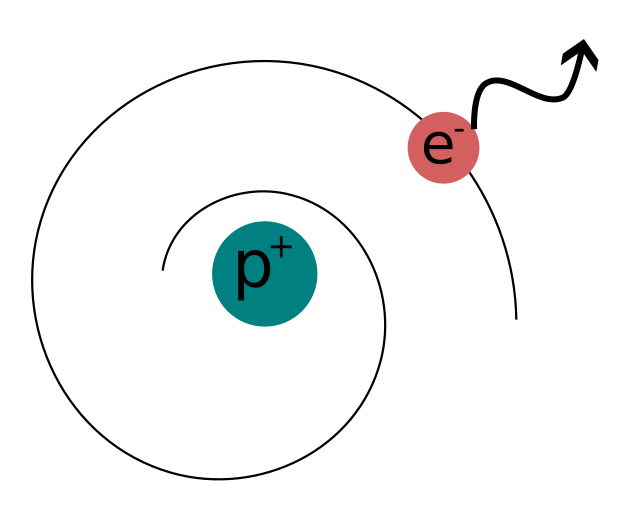
\includegraphics[width=0.2\linewidth]{../figures/intro/class_electron.png}
      \hfill
      \only<3->{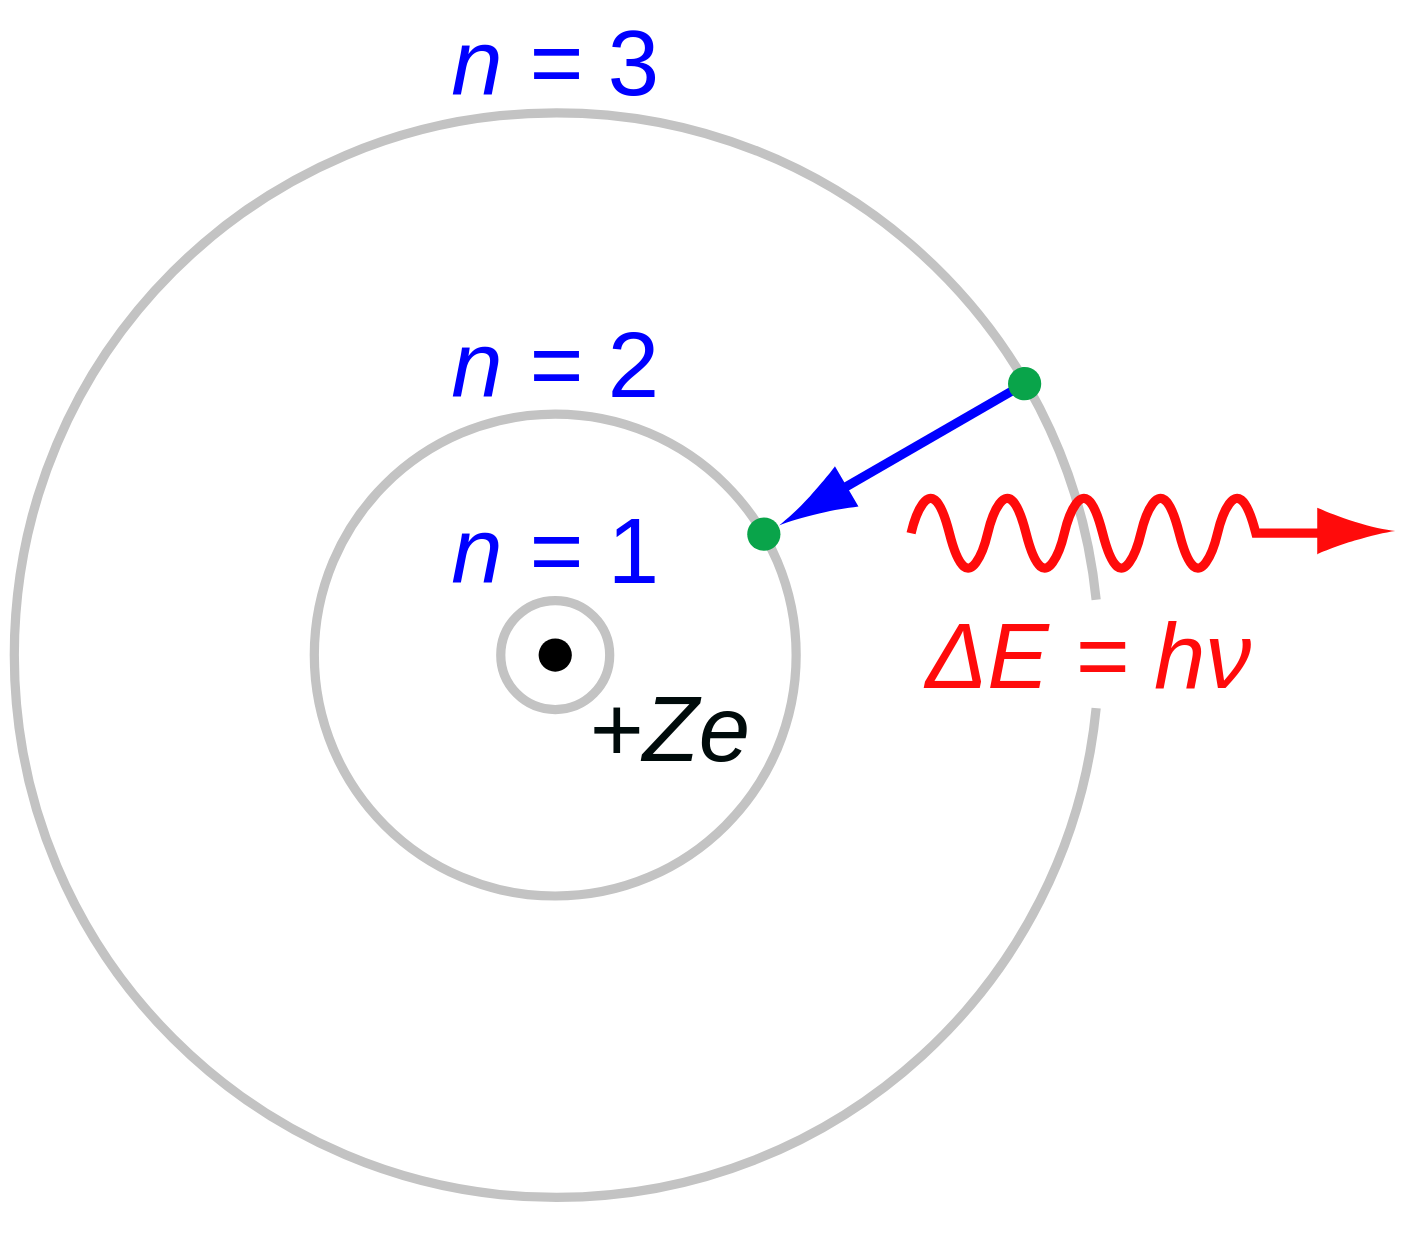
\includegraphics[width=0.2\linewidth]{../figures/intro/bohr_model.png}}
    \end{figure}
    \item Yet matter does not collapse, it is stable.\\~\\
    \item Quantum mechanics: stable minimum energy level + quantized energy levels: Bohr model (1910s).\\~\\
    \item Transitions occur in precise energy packets (photons).
  \end{itemize}
\end{frame}

\begin{frame}{Spectral lines}
  \begin{itemize}[<+->]
    \item Emission spectrum of the Sun (Fraunhofer, 1814).
    \begin{figure}
      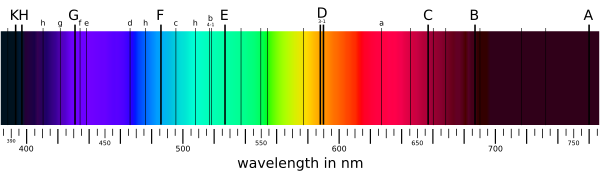
\includegraphics[width=0.6\linewidth]{../figures/intro/Fraunhofer_lines.png}
    \end{figure}
    \item Dark lines due to absorption by gases in the Sun and our atmosphere (Bunsen and Kirchhoff, 1859).
    \\~\\
    \item Spectral lines are the signatures of these discrete jumps between orbitals (Bohr).
  \end{itemize}
\end{frame}

\begin{frame}{Electron diffraction (1927)}
  \begin{itemize}
    \item Electrons pass through two slits. Classically, one expects two bands.
  \end{itemize}
\end{frame}

\begin{frame}{Electron diffraction (1927)}
  \begin{itemize}[<+->]
    \item Electrons pass through two slits. Classically, one expects two bands.
    \item Even when sent one at a time, the interference pattern appears -- just like for light waves (Young, 1801).
    \begin{figure}
      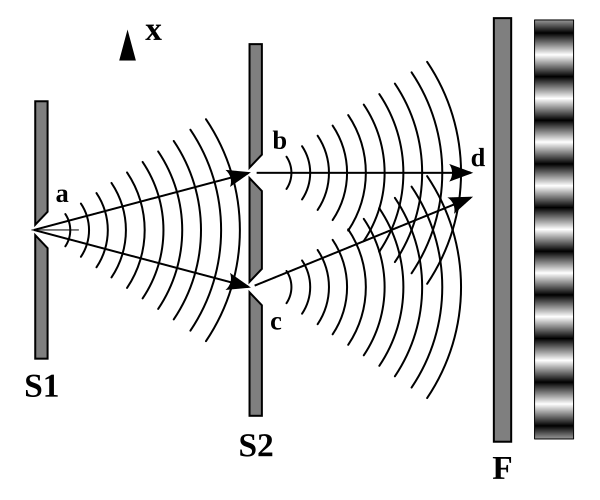
\includegraphics[width=0.3\linewidth]{../figures/intro/fente_Young.png}
    \end{figure}
    \item Classical mechanics cannot explain the wave-like behaviour of matter.
    \item Each electron \textbf{interferes with itself} because it passes through both slits 
    \textbf{at the same time}. It is in two places at the same time, so we don't know exactly where.
  \end{itemize}
  \vfill
  \hfill\href{https://www.youtube.com/watch?v=JlsPC2BW_UI&list=PL_wN0FeVwhX6yH4bIQdHEvuPAQqWJM84M}{Young's slits video}
\end{frame}

\begin{frame}{Stern-Gerlach experiment (1922)}
  \begin{itemize}[<+->]
    \item Beam of silver atoms in an inhomogeneous magnetic field.
    \\~\\
    \begin{figure}
      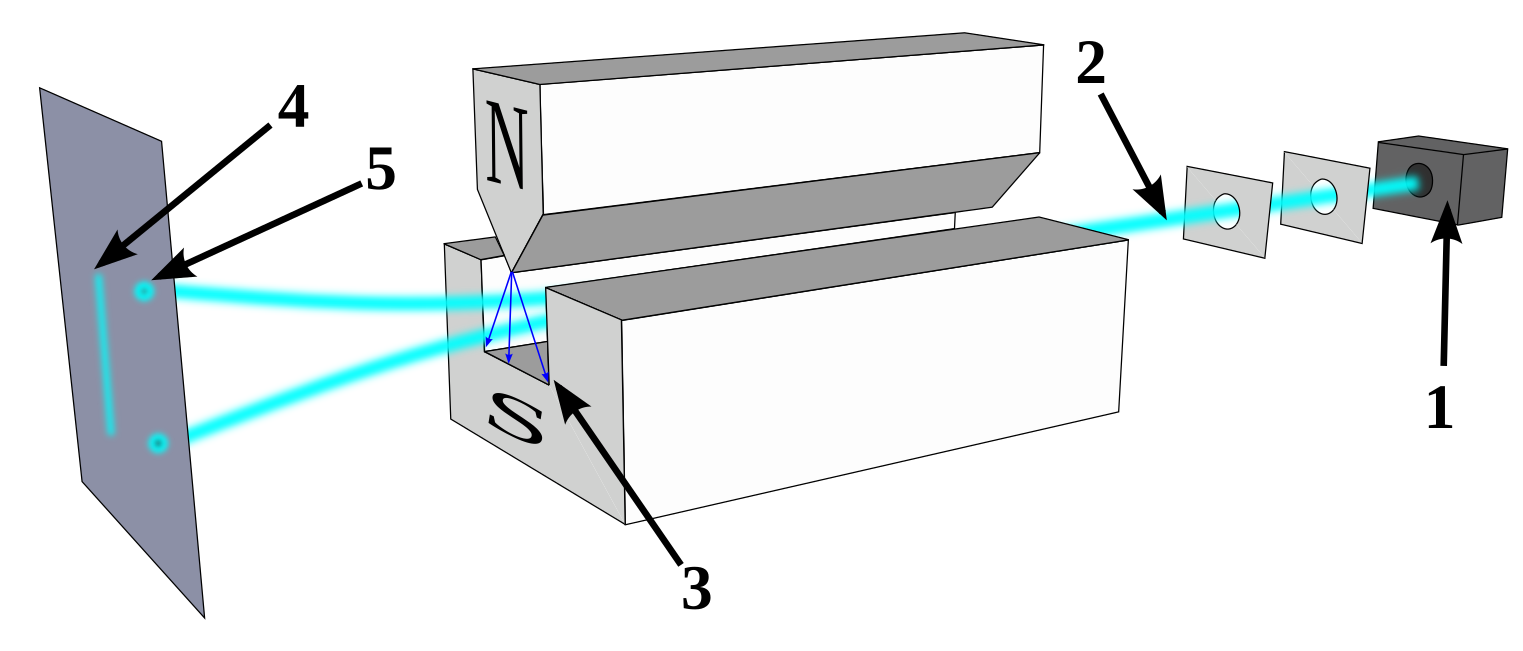
\includegraphics[width=0.45\linewidth]{../figures/intro/stern-gerlach.png}
    \end{figure}
    \item Separation into two distinct spots: the spin measurement yields quantized values.
    \item Discrete nature of quantum observables.
    \item Idea of a \textbf{two-level system}
  \end{itemize}
  \vfill
  \hfill\href{https://www.youtube.com/watch?v=8wS4IOzAhFA&list=PL_wN0FeVwhX6yH4bIQdHEvuPAQqWJM84M&index=5}{Stern-Gerlach video}
\end{frame}

\begin{frame}{Major consequences}
  \begin{itemize}
    \item Discrete energy levels + spin $\quad \rightarrow \quad$ two-level systems.
    \\~\\
    \item Superposition of states.
    \\~\\~\\~\\
  \end{itemize}
\end{frame}

\begin{frame}{Major consequences}
  \begin{itemize}
    \item Discrete energy levels + spin $\quad \rightarrow \quad$ two-level systems.
    \\~\\
    \item Superposition of states.
    \\~\\~\\~\\
    \centering
    \textbf{Building blocks leading to quantum computing}\\~\\
    Qubit = two-level quantum system
  \end{itemize}
\end{frame}

\begin{frame}{Superposition: more information per qubit}
    \begin{itemize}[<+->]
        \item Computation represented as an operation on a sequence of bits $(b_3 b_2 b_1)$
        \item A classical computer operates on one sequence at a time: %$(b_n,\cdots,b_2,b_1) \longrightarrow f(b_n,\cdots,b_2,b_1)$
        \begin{align*}
            (101) \longrightarrow f(101)
        \end{align*}
        \item A quantum computer can encode all possible sequences in a single state and operate on all sequences in a single operation:
        \begin{align*}
            \begin{Bmatrix}
                (000) \\ (001) \\ (010) \\ \cdots \\ (111)
            \end{Bmatrix}
            \quad \longrightarrow \quad
            \begin{Bmatrix}
                f(000) \\ f(001) \\ f(010) \\ \cdots \\ f(111)
            \end{Bmatrix}
        \end{align*}
        \item \textbf{Problem}: we can only retrieve \textbf{one of the results per computation}. The measurement must be repeated a number of times to \textbf{find the most probable answers}.
    \end{itemize}
\end{frame}

\section{Why use quantum computers?}

\begin{frame}{Superposition: more information per qubit}
  \begin{columns}[T,onlytextwidth]
    \column{0.48\textwidth}
    \textbf{Classical}\\
    \begin{itemize}
      \item To encode 0, 1, 2, 3 each must be written in two bits.
      \item A register contains only one state at a time.
    \end{itemize}
    \column{0.48\textwidth}
    \textbf{Quantum}\\
    \begin{itemize}
      \item Two qubits suffice: $\ket{\psi}$ can superpose 00, 01, 10, 11.
      \item All these states are manipulated simultaneously before measurement.
    \end{itemize}
  \end{columns}
\end{frame}


\begin{frame}{Fundamental differences between classical and quantum computers}
  \centering
  \begin{tabular}{l|c|c}
    & Classical & Quantum \\\hline
    ~& ~ & ~\\
    Encoding & Bit (0 \textbf{or} 1) & Qubit (0 \textbf{and} 1) \\
     ~& ~ & ~\\
    Logic gates & Boolean & Matrix-based \\
    ~& ~ & ~\\
    Sensitivity to environment & Low & High \\
    ~& ~ & ~\\
    Knowledge of result & Deterministic & Probabilistic \\
  \end{tabular}
\end{frame}

\begin{frame}{Usefulness despite this limitation}
  \begin{itemize}
    \item {\bf Grover's algorithm:} Quadratic speedup for searching a solution to a ``black box'' function. Applications: searching an element in an unstructured database, inverting a hash function, solving an NP-complete problem, ... \\~\\
    \item {\bf Shor's algorithm:} Exponential speedup of number factorization (breaks RSA encryption). Based on a quantum algorithm accelerating the computation of the {\bf Fourier transform}, a mathematical technique very useful in many fields. \\~\\
    \item {\bf Hybrid optimization algorithms (QAOA, VQE,...):} Main applications in chemistry, quantum advantage still debated.
  \end{itemize}
\end{frame}

\begin{frame}{What we offer}
  
  \begin{itemize}
    \setlength{\itemsep}{0.8em}
    \item Qubit: bra-ket and vector representations
    \item Quantum logic gates and matrix representation
    \item Hands-on programming with Qiskit
    \item Measuring a qubit state + Quantum key distribution
    \item Multi-qubit systems + Quantum teleportation
    \item Grover's algorithm
    \item Physical platforms for building quantum computers
    \item Possibility to discuss further topics to go deeper...
  \end{itemize}
\end{frame}

\end{document}
